Chương này trình bày cơ sở lý thuyết và các công nghệ nền tảng phục vụ cho việc nghiên cứu và triển khai giải pháp định tuyến. Nội dung bao gồm tổng quan về mạng cảm biến không dây và mạng ad-hoc, các thuật toán định tuyến phổ biến cùng với thuật toán định tuyến dựa trên Gradient. Ngoài ra, chương cũng giới thiệu về giao thức Bluetooth Low Energy Mesh và vi xử lý nRF54L15 của Nordic Semiconductor.

\section{Tổng quan về mạng cảm biến không dây}

Mạng cảm biến không dây (Wireless Sensor Network - WSN) là một hệ thống bao gồm nhiều node cảm biến có khả năng thu thập dữ liệu từ môi trường xung quanh và truyền thông tin về trạm gốc (Base station) thông qua kết nối không dây. Với sự phát triển của công nghệ vi điện tử và truyền thông không dây, WSN đã trở thành một trong những công nghệ nền tảng quan trọng trong lĩnh vực Internet of Things (IoT), được ứng dụng rộng rãi trong các vấn đề như giám sát môi trường, nông nghiệp thông minh, quản lý tòa nhà và y tế.

\subsection{Kiến trúc mạng cảm biến không dây}

Kiến trúc của mạng cảm biến không dây thường bao gồm ba thành phần chính: các node cảm biến (sensor nodes), trạm gốc (base station/sink node) và giao thức truyền thông như trong hình \ref{fig:WSN}. Các node cảm biến có vai trò giám sát và thu thập dữ liệu môi trường như nhiệt độ, độ ẩm, ánh sáng hoặc các thông số khác. Dữ liệu thu thập được sẽ được truyền về trạm gốc thông qua các giao thức truyền thông, có thể thông qua một hoặc nhiều node trung gian, để đến trạm gốc. Tại đây, dữ liệu được xử lý, lưu trữ hoặc chuyển tiếp đến các hệ thống giám sát và điều khiển.

\begin{figure}[h!]
    \centering
    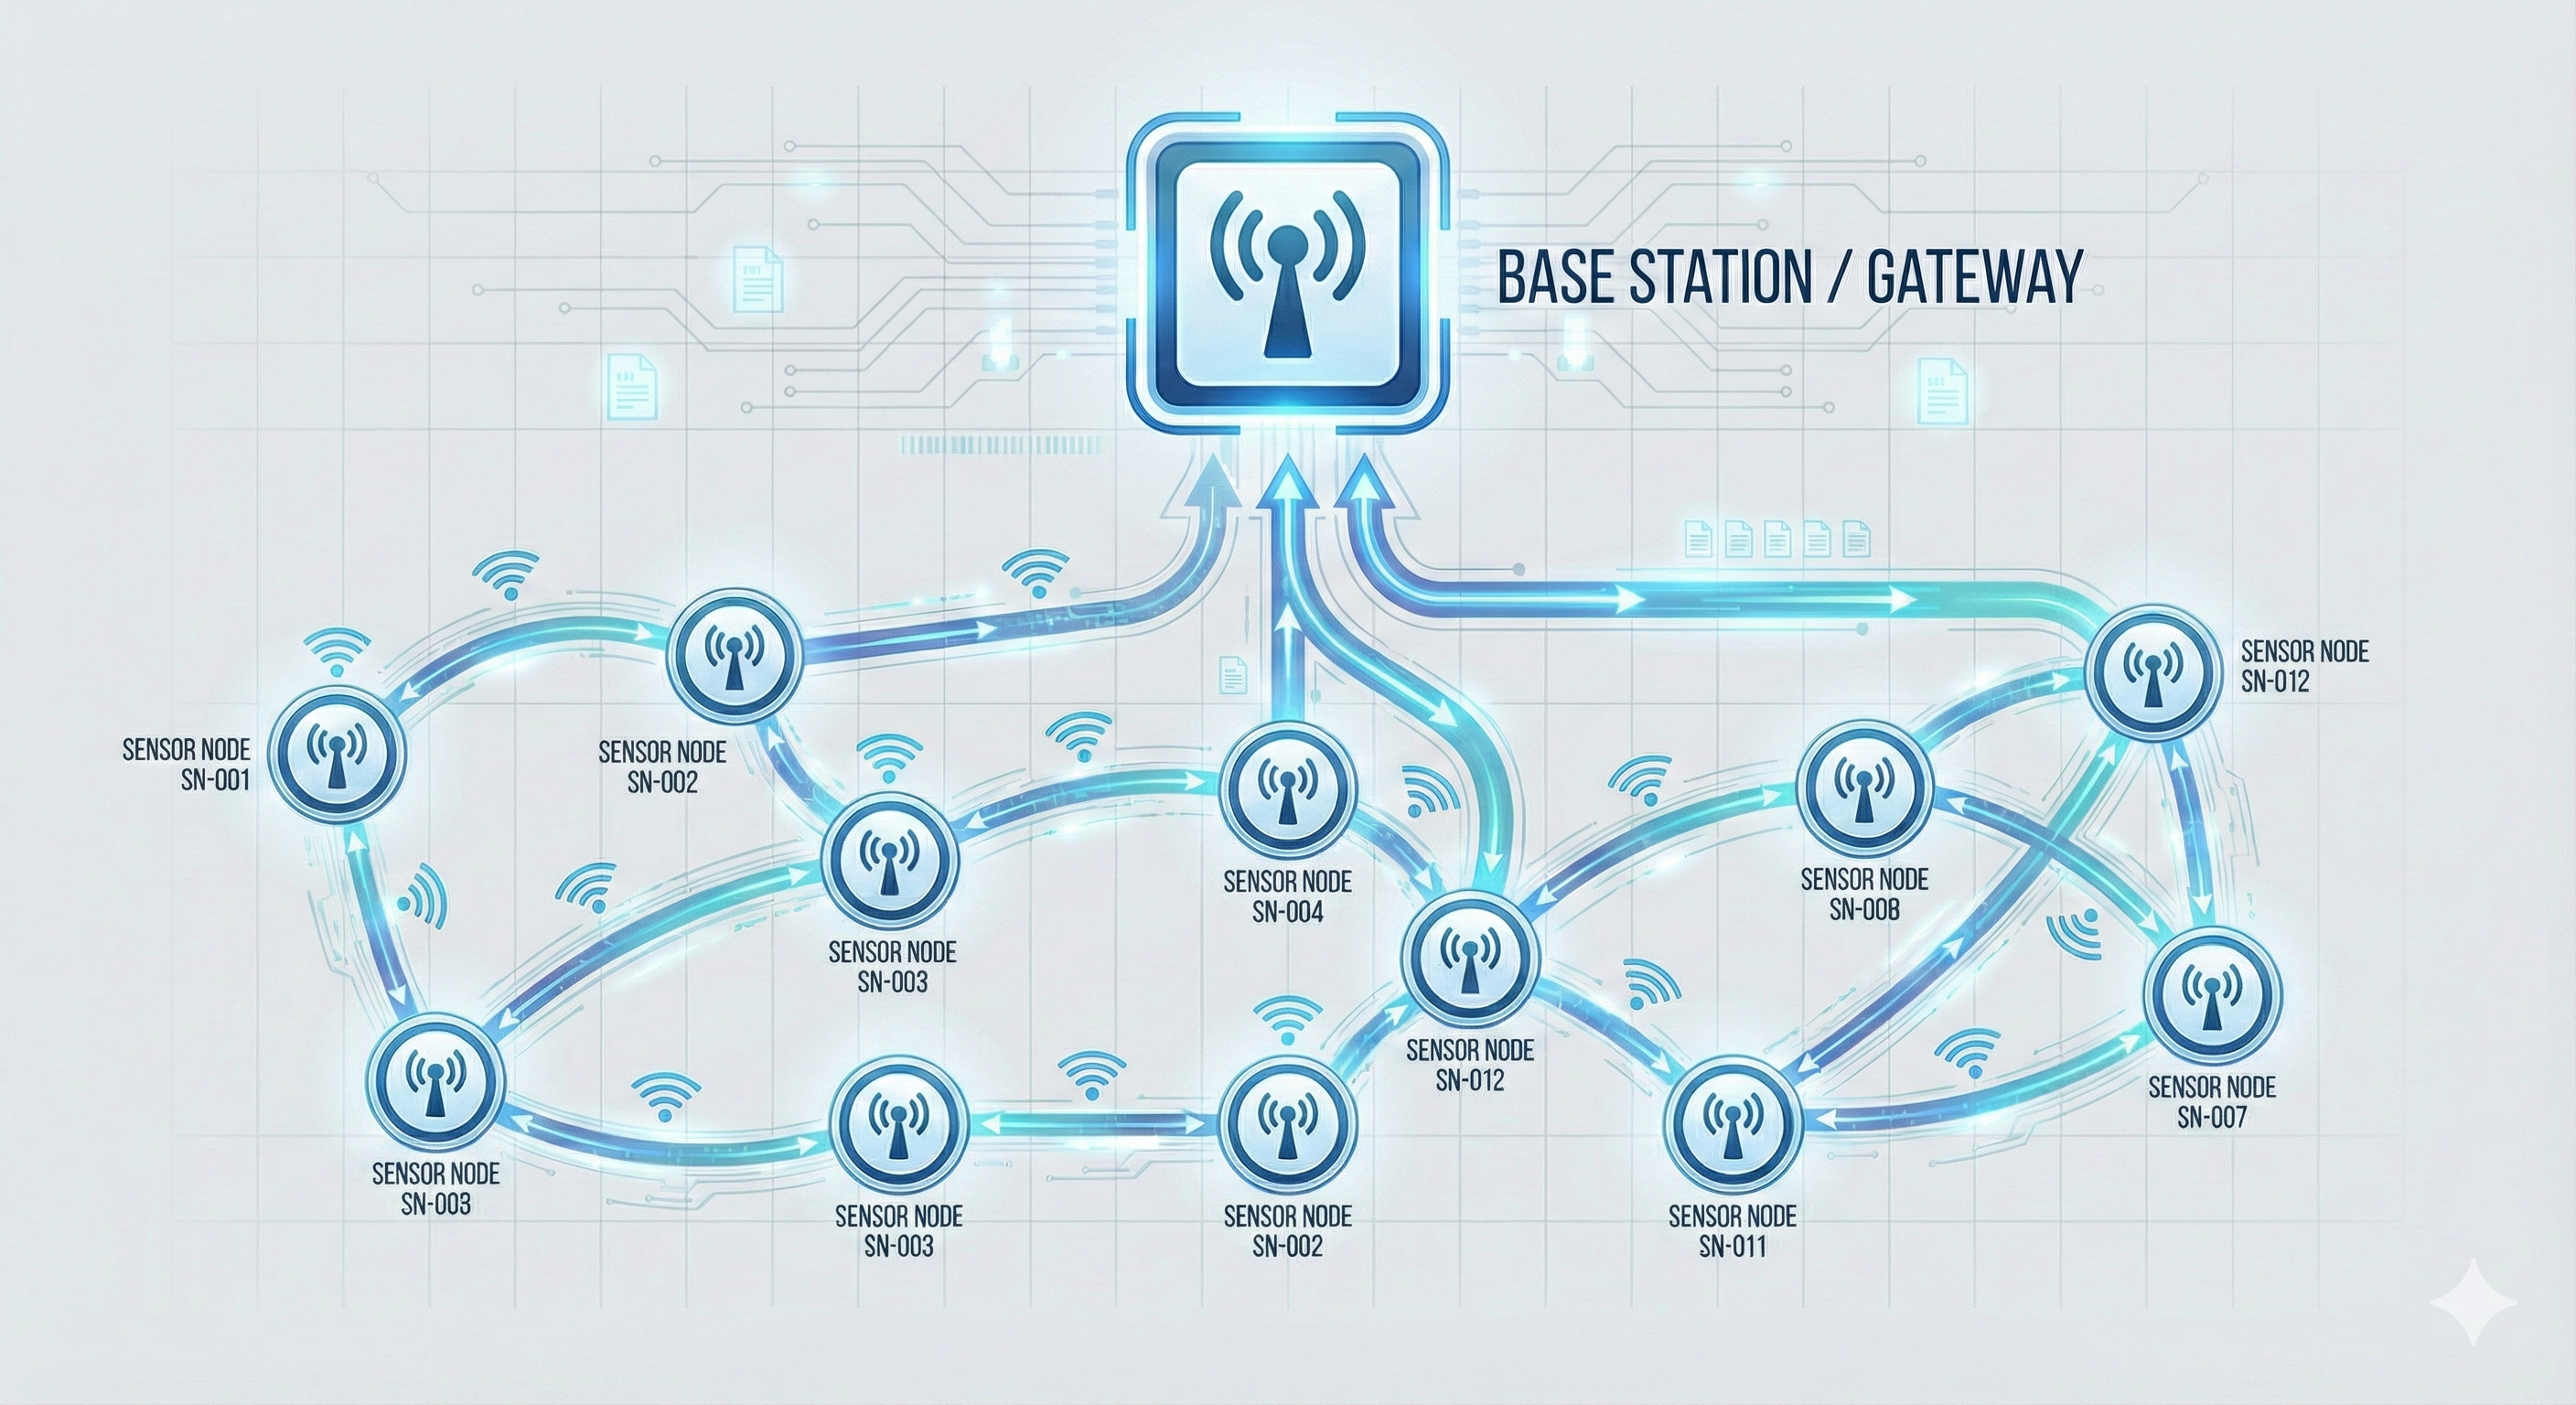
\includegraphics[width=1\textwidth]{chapter3/image/WSN.png}
    \caption{Kiến trúc mạng cảm biến không dây}
   \label{fig:WSN}
\end{figure}

\subsection{Các thành phần của node cảm biến}

Một node cảm biến điển hình bao gồm bốn thành phần cơ bản: khối cảm biến (sensing unit), khối xử lý (processing unit), khối truyền thông (communication unit) và khối nguồn (power unit) như trong hình \ref{fig:Node}. Khối cảm biến có nhiệm vụ thu thập dữ liệu từ môi trường và chuyển đổi thành tín hiệu điện. Khối xử lý thực hiện các tác vụ xử lý dữ liệu, điều khiển hoạt động của node và thực thi các giao thức truyền thông. Khối truyền thông đảm nhận việc gửi và nhận dữ liệu qua sóng vô tuyến. Khối nguồn cung cấp năng lượng cho toàn bộ node, thường là pin hoặc nguồn năng lượng thu hoạch từ môi trường.

\begin{figure}[h!]
    \centering
    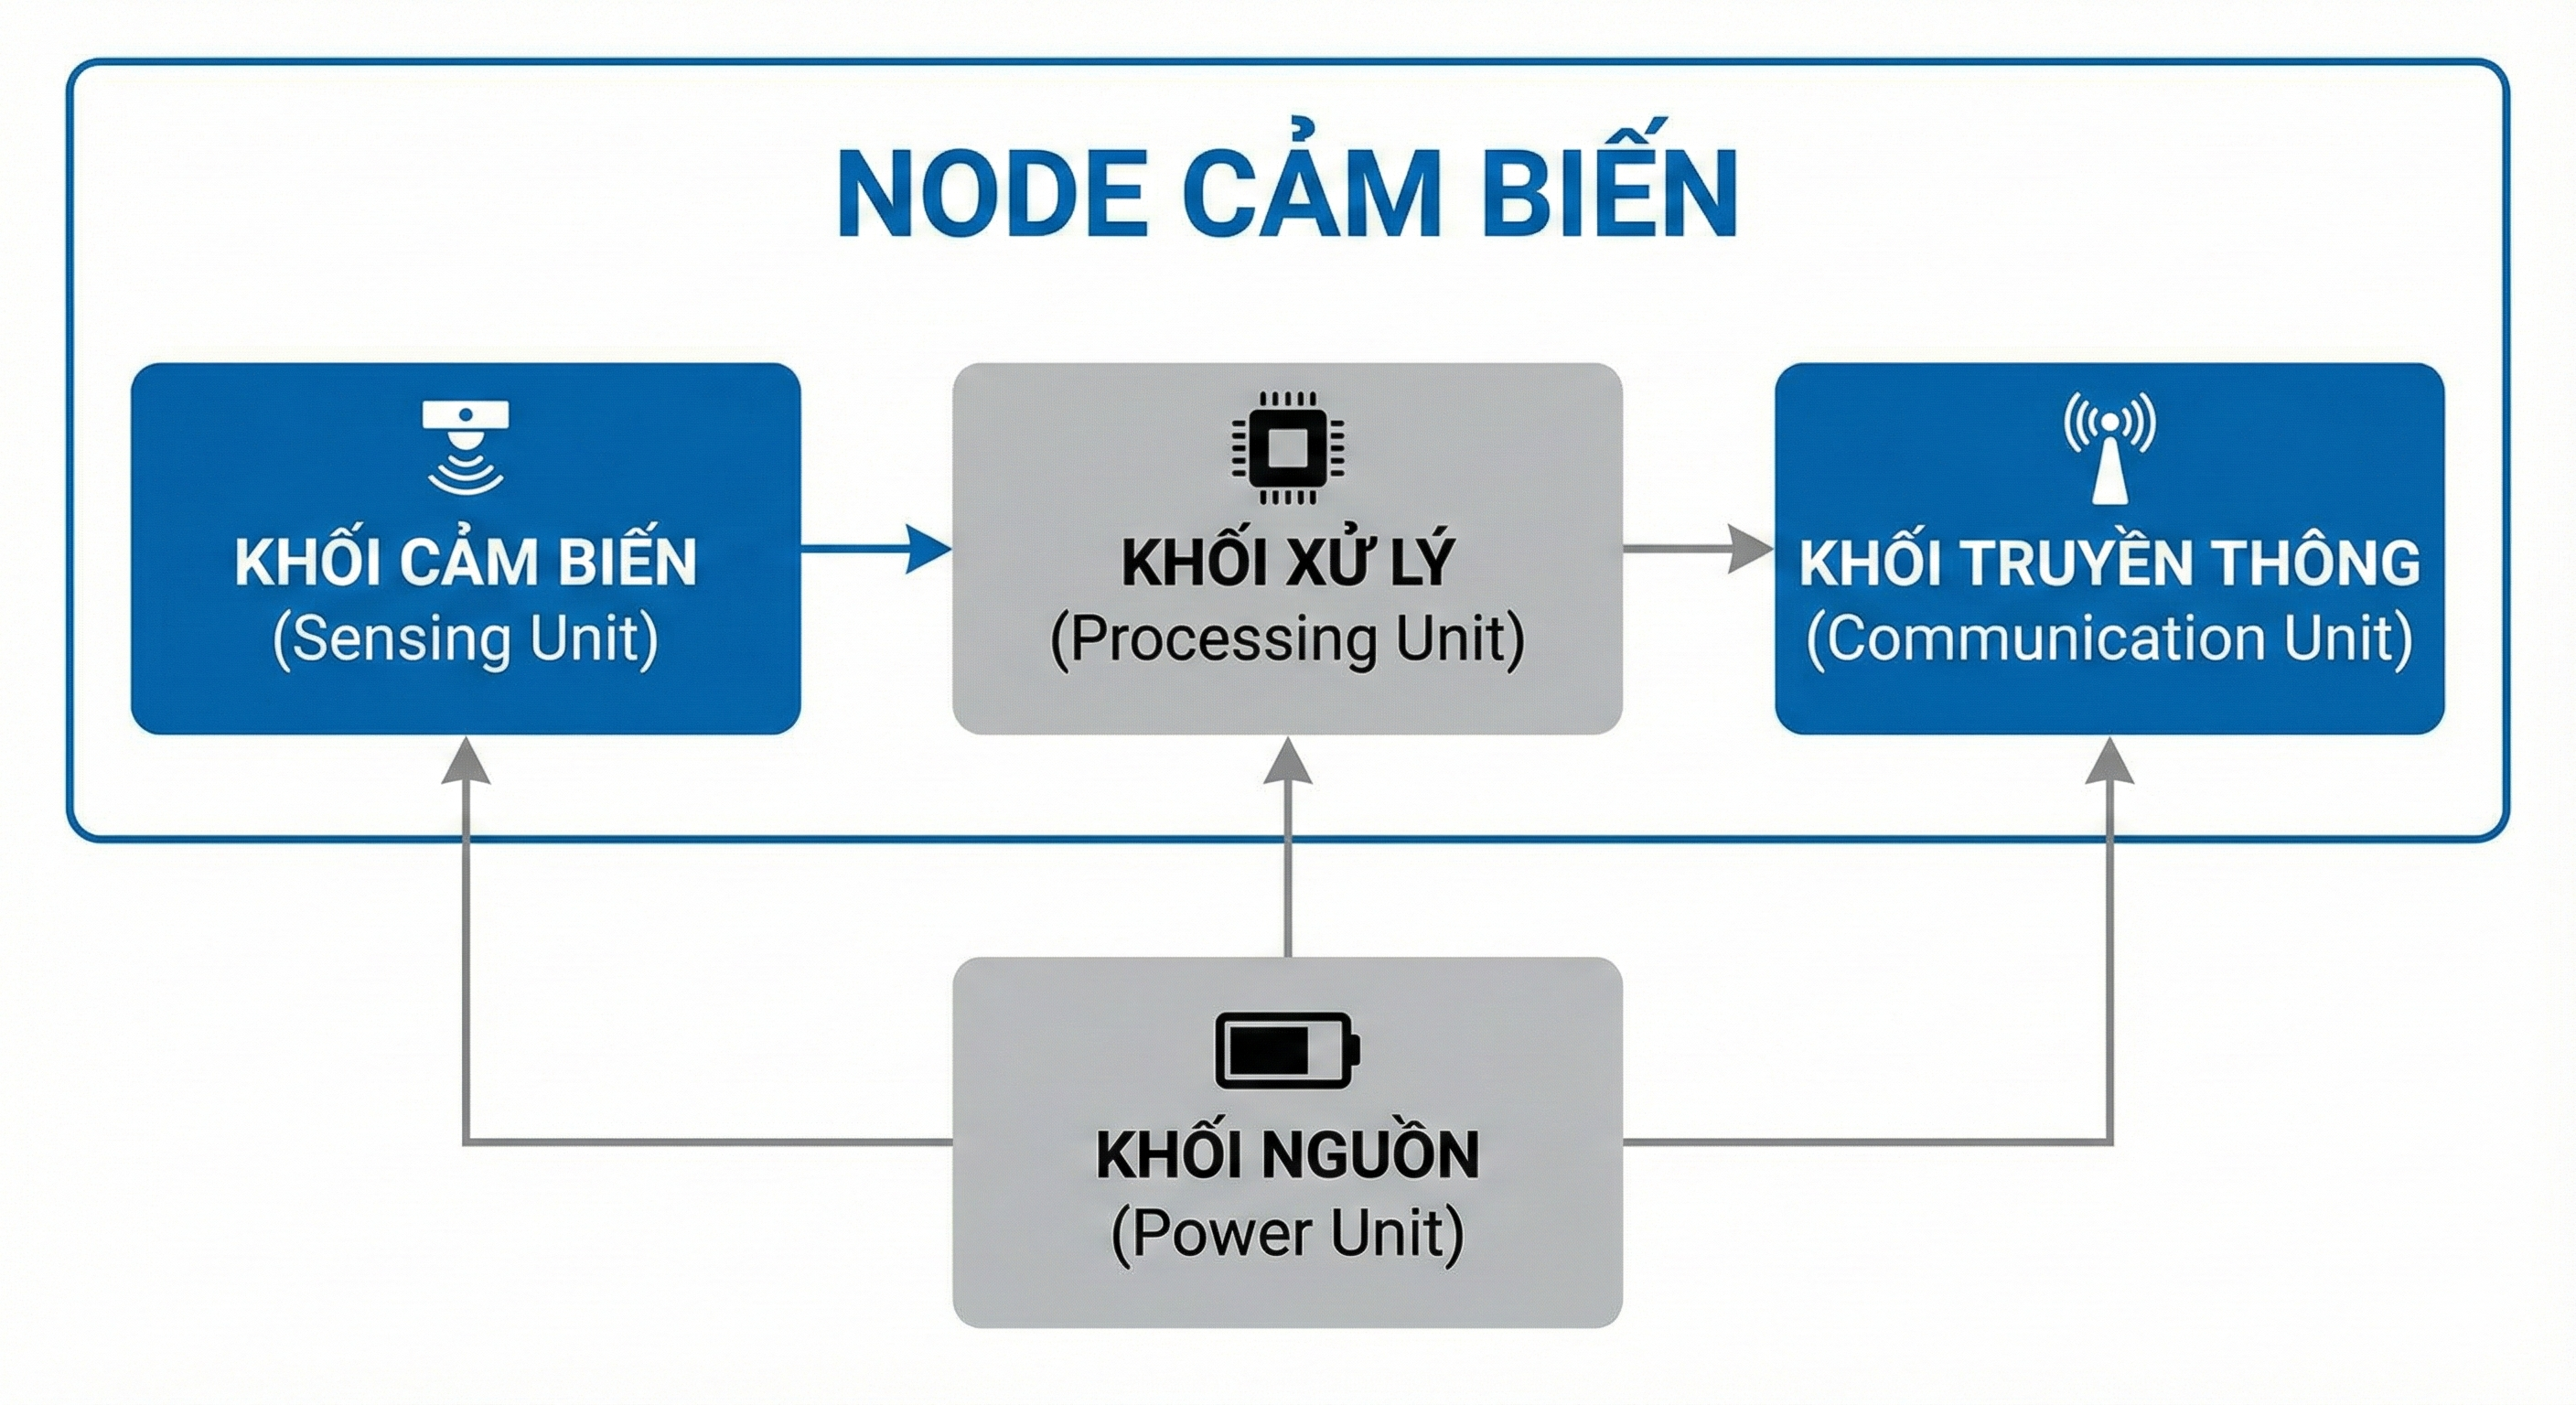
\includegraphics[width=1\textwidth]{chapter3/image/Node.png}
    \caption{Thành phần của một node cảm biến}
   \label{fig:Node}
\end{figure}

\subsection{Đặc điểm và hạn chế của WSN}

Mạng cảm biến không dây có một số đặc điểm nổi bật như khả năng triển khai linh hoạt, chi phí thấp và khả năng tự tổ chức. Tuy nhiên, WSN cũng đối mặt với nhiều hạn chế đáng kể. Thứ nhất, các node cảm biến thường có nguồn năng lượng hạn chế do sử dụng pin, đòi hỏi các giải pháp tiết kiệm năng lượng trong thiết kế phần cứng và phần mềm. Thứ hai, khả năng xử lý và bộ nhớ của node bị giới hạn, ảnh hưởng đến việc triển khai các thuật toán phức tạp. Cuối cùng, băng thông truyền thông không dây có giới hạn, yêu cầu các giao thức truyền thông hiệu quả. Những hạn chế này đặt ra thách thức lớn trong việc thiết kế các thuật toán định tuyến cho WSN, đòi hỏi sự cân bằng giữa hiệu suất và mức tiêu thụ tài nguyên.
